\chapter*{Anexo I: Hazlo tú mismo}
\label{cap:anexoi}

\noindent En este anexo se explica, paso a paso, todo lo necesario para poder reproducir y utilizar este robot a partir del contenido 
existente en el repositorio\footnote{\url{https://github.com/RoboticsURJC/tfg-vperez.git}} de este proyecto.

\section*{Obtención de los ficheros STL}
\noindent Para poder imprimir las distintas piezas, primeramente se requiere obtener los ficheros STL a partir de los ficheros fuente (piezas de FreeCAD) . 
Estos, los podemos encontrar en la carpeta \textbf{/src/design/FreeCad} del proyecto. Para generarlos se deben realizar los siguientes pasos:
\begin{enumerate}
\item Abrimos la pieza correspondiente con FreeCAD (pulsando encima de ella).
\item Cambiamos al banco de trabajo \textit{Mesh Design}.
\item Hacemos click sobre la pieza para seleccionarla y, posteriormente, pulsamos el botón \textit{Crear malla de forma} del panel superior.
\item Introducimos un valor de superficie de desviación de 0.01mm y damos en OK.
\item Click derecho del ratón sobre el objeto de malla creado y exportamos la malla con el botón \textit{Exportar malla}. 
\end{enumerate}

\begin{tcolorbox}[colback=blue!5!white,colframe=blue!75!black,title=Nota]
    No se recomienda generar directamente el STL con la opción de exportar del menú superior debido a que no se puede controlar la cantidad de polígonos 
    de la malla y por defecto es bastante baja.
\end{tcolorbox}

Una vez obtenidos todos los ficheros STL, se pueden importar en el laminador, en este caso se ha empleado 
Ultimaker Cura 5.2.1 para generar los ficheros que entiende la impresora 3D. La densidad requerida para cada pieza 
y la cantidad de ellas, se pueden ver en el Cuadro 5.8 del Capítulo 5.

\newpage
\section*{Montaje}
\noindent Actualmente, no se dispone de una guía detallada de montaje. Aún así el montaje resulta bastante sencillo 
e intuitivo. La manera recomendada de proceder es fijándose en el fichero de 
montaje llamado \textit{\#0\_ASSEMBLY.FCStd} que se encuentra en la misma carpeta que las piezas. En él 
aparece cada pieza, su posición y nombre. En la Sección 5.6 se puede ver la lista de las piezas que 
son necesarias para poder comprarlas o fabricarlas.

\section*{Software}
\noindent Todo el software necesario para hacer funcionar este robot se encuentra en la carpeta \textbf{/src/software} del repositorio. Dentro de 
ella existen una serie de paquetes para utilizar el robot, los cuales son:
\begin{itemize}
\item Paquete \textbf{\textit{g\_arm}}: Es un paquete de ROS 2 que contiene el software necesario para comunicarse con el robot desde el 
ecosistema ROS. Dentro de él se encuentra la carpeta \textbf{\textit{g\_arm\_lib}} con las clases de python necesarias para abstraer al 
ejecutable (driver del robot) de las comunicaciones.
\item Paquete \textbf{\textit{g\_arm\_description}}: Es un paquete de descripción creado para representar el robot real en el mundo virtual. No contiene código, únicamente una serie de lanzadores para poder visualizarlo.
\item Paquete \textbf{\textit{g\_arm\_moveit2}}: Es un paquete de MoveIt 2 que utiliza el anterior paquete para poder controlar el robot 
real desde este framework.
\item Paquete \textbf{\textit{g\_arm\_python\_examples}}: Es un paqute que contiene ejemplos de código para mover el robot mediante la API de PyMoveit2.
\end{itemize}

\begin{tcolorbox}[colback=blue!5!white,colframe=blue!75!black,title=Nota]
    Aunque es posible controlar las articulaciones del robot a bajo nivel enviando órdenes de código G por el puerto serie, se pierde la 
posibilidad de conocer la posición absoluta 
de cada articulación. Debido a esto, es recomendable utilizar al menos la capa de abstracción \textit{Robot} que se puede encontrar en 
la carpeta \textbf{\textit{g\_arm\_lib}} del paquete \textbf{\textit{g\_arm}}. Para conocer su funcionamiento, se puede analizar el código del ejecutable 
\textit{driver.py} de esa misma carpeta. 
\end{tcolorbox}

Aun así, lo ideal es utilizar ROS 2 Humble y MoveIt 2 para controlar el robot. Para ello, es necesario tener instalado 
ambos y hacer uso de los cuatro paquetes mencionados.

\newpage
Para utilizar estos paquetes es necesario añadirlos al \textit{workspace} y compilar. En caso de que no se tenga uno, 
se deben seguir los siguientes pasos: 
\begin{enumerate}
\item Se crea una carpeta llamada \textit{workspace} en el directorio \textit{home}, por ejemplo. Dentro de ella 
se debe de crear la carpeta \textit{src}. 
\item En \textit{src}, se copian los paquetes mencionados anteriormente. Además de estos cuatro, es necesario incluir el paquete 
PyMoveit2\footnote{\url{https://github.com/AndrejOrsula/pymoveit2}}.
\item Desde el nivel de la carpeta \textit{workspace} ejecutamos el comando \mbox{\textit{colcon build --merge-install --symlink-install}}.
\item Para que ROS lo encuentre debemos añadir la siguiente línea al final del fichero oculto \textit{.bashrc} del directorio \textit{home}:
\textbf{source \textasciitilde/workspace/install/setup.bash}

\end{enumerate}

La estructura del \textit{workspace} debería quedar igual a la mostrada en la Figura \ref{fig:ws_tree}.
\begin{figure} [ht!]
    \begin{center}
        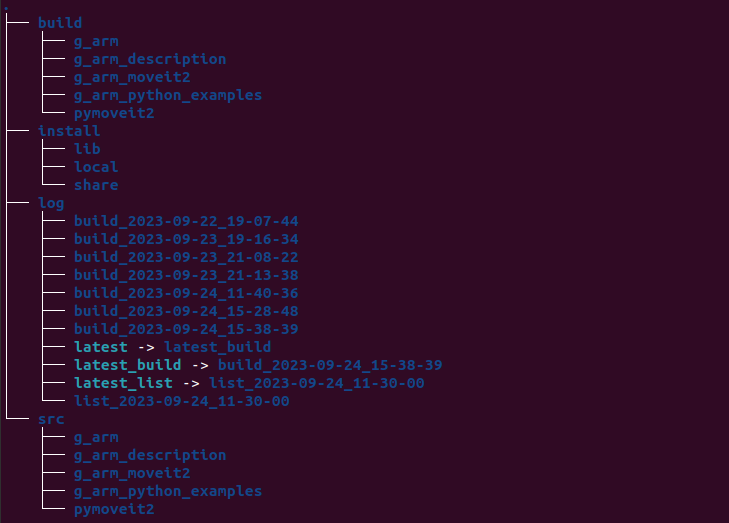
\includegraphics[width=11cm]{figs/ws_tree.png}
    \end{center}
    \caption{Resultado de ejecutar \textit{tree -d -L 1} en la carpeta \textit{workspace}}.
\label{fig:ws_tree}
\end{figure}

En cuanto al firmware interno del robot, utiliza la versión de Grbl v1.1. Existen numerosas guías en internet de 
cómo instalarlo. En el caso de utilizar la misma placa de este proyecto, no es necesario instalar nada ya que viene preinstalado de fábrica. Lo único 
a cambiar son los parámetros internos a los mostrados en el Cuadro 6.2. En esa misma sección se detalla como se cambian.

